% mnras_template.tex
%
% LaTeX template for creating an MNRAS paper
%
% v3.0 released 14 May 2015
% (version numbers match those of mnras.cls)
%
% Copyright (C) Royal Astronomical Society 2015
% Authors:
% Keith T. Smith (Royal Astronomical Society)

% Change log
%
% v3.0 May 2015
%    Renamed to match the new package name
%    Version number matches mnras.cls
%    A few minor tweaks to wording
% v1.0 September 2013
%    Beta testing only - never publicly released
%    First version: a simple (ish) template for creating an MNRAS paper

%%%%%%%%%%%%%%%%%%%%%%%%%%%%%%%%%%%%%%%%%%%%%%%%%%
% Basic setup. Most papers should leave these options alone.
\documentclass[fleqn,usenatbib,letters]{mnras}%added "letters", a4paper is default

% MNRAS is set in Times font. If you don't have this installed (most LaTeX
% installations will be fine) or prefer the old Computer Modern fonts, comment
% out the following line
%\usepackage{newtxtext,newtxmath}
% Depending on your LaTeX fonts installation, you might get better results with one of these:
\usepackage{mathptmx}
%\usepackage{txfonts}

% Use vector fonts, so it zooms properly in on-screen viewing software
% Don't change these lines unless you know what you are doing
\usepackage[T1]{fontenc}
\usepackage{ae,aecompl}


%%%%% AUTHORS - PLACE YOUR OWN PACKAGES HERE %%%%%

% Only include extra packages if you really need them. Common packages are:
\usepackage{graphicx}	% Including figure files
\usepackage{amsmath}	% Advanced maths commands
\usepackage{amssymb}	% Extra maths symbols
\usepackage{cases}  %define a step function

%%%%%%%%%%%%%%%%%%%%%%%%%%%%%%%%%%%%%%%%%%%%%%%%%%

%%%%% AUTHORS - PLACE YOUR OWN COMMANDS HERE %%%%%


%%%%%%%%%%%%%%%%%%%%%%%%%%%%%%%%%%%%%%%%%%%%%%%%%%

%%%%%%%%%%%%%%%%%%% TITLE PAGE %%%%%%%%%%%%%%%%%%%

% Title of the paper, and the short title which is used in the headers.
% Keep the title short and informative.
\title[]{Testing for Flaring Star-Planet Interactions in AU Mic TESS Observations}

% The list of authors, and the short list which is used in the headers.
% If you need two or more lines of authors, add an extra line using \newauthor
\author[E. Ilin et al.]{
E. Ilin$^{1,2}$,\thanks{E-mail: eilin@aip.de}
K. Poppenhaeger$^{1,2}$,
\\
% List of institutions
$^{1}$Leibniz-Institute for Astrophysics Potsdam (AIP), An der Sternwarte 16, 14482 Potsdam, Germany\\
$^{2}$Institute for Physics and Astronomy, University of Potsdam, Karl-Liebknecht-Str. 24/25, 14476 Potsdam, Germany
}

% These dates will be filled out by the publisher
\date{Accepted XXX. Received YYY; in original form ZZZ}

% Enter the current year, for the copyright statements etc.
\pubyear{2020}

% Don't change these lines
\begin{document}
\label{firstpage}
\pagerange{\pageref{firstpage}--\pageref{lastpage}}
\maketitle

% Abstract of the paper
\begin{abstract}
Magnetically active stars with close-in planets are expected to show signs of magnetic star-planet interaction in form of a modulation of magnetic activity with the orbital phase of the planet. However, the magnitude of this interaction proves difficult to constrain.

In this study we searched the optical light curves of the young, active M1 star AU Mic for signs of flaring SPI with its innermost planet. We find that the flare occurrence rates are consistent with a uniform distribution of flares across the stellar surface with respect to stellar rotation phase. We find marginal deviation with orbital phase, but cannot make firm conclusions since the TESS light curves only cover about 5 orbital periods of AU Mic b. 
\end{abstract}

% Select between one and six entries from the list of approved keywords.
% Don't make up new ones.
\begin{keywords}
keyword1 -- keyword2 -- keyword3
\end{keywords}

%%%%%%%%%%%%%%%%%%%%%%%%%%%%%%%%%%%%%%%%%%%%%%%%%%
%
%-------------------------------------------------------------------

\section{Introduction}

Stellar flares are known as electromagnetic explosions in the stellar coronae that are driven by the dynamics of the surface magnetic fields. As such, they are phenomena triggered intrisically by the star. Another class of flares, though phenomenologically the same, are flares triggered by magnetic star-planet interaction (SPI).

In such flares, the energy for the flare is provided by XXXX, and the event itself is triggered by the re-connection of stellar and planetary magnetic field lines. For this to occur, the planet must revolve around the star in close orbit, so that it moves within the stellar Alfven zone for at least a fraction of its orbit. When the planet is within the Alfven zone, the magnetic field and the energy transported along the field lines as particles or waves can fall back on to the star, whereas outside of it i woudl be carried away by the stellar wind. 

\textit{Do we need Prot and Porb to be different actually?}

When re-connection between star and planet occurs, the energy channelled back into the stellar atmosphere can create an activity hot spot (XXXX Halpha? Xray?) trigger a flare. The footpoint of the connecting field line is expected to move with the planetary orbit (but need not neccessarily be the sub-planetary point).



However, the exact phase function and magnitude of SPI as it manifests in flares is an open question. \citet{maggio2015} report the observation of an X-ray flare and enhanced chromospheric activity right after periastron of the eccentric Hot Jupiter system HD 17156, but lin light of other (fruitless) searches for excess flares in similar systems~\citep{figueira2016}, the interpretation as SPI remains very suggestive. 

One interpretation is that the interaction is so weak that the system has to be observed for a long time before the SPI flares become measurable against the background of intrinsic flares. \citet{fischer2019} searched for orbital modulation of flare occurrence with the innermost planets of the seven-planet TRAPPIST-1, but found modest hints at best. 

Recently, AU Mic has been shown to be a promising candidate for such magnetic SPI. 


\subsection{AU Mic}
Rotation period $4.862\pm 0.032$ d~\citep{martioli2021}, $4.863\pm 0.001$ d~\citep{plavchan2020}

AU Mic is a member of the $\beta$ Pic young moving group, which is $16-29$ Myr old~\citep{malo2014,binks2014,mamajek2014,bell2015,binks2016,shkolnik2017,miretroig2020}. Based on its lithium abundance, AU Mic could be a few Myr older than the average group member~\citep{malo2014}. 

%Spectral type tends to agree on M1, but effective temperature is lower in Plavchan et al. (2009)
AU Mic shows strong differential rotation (XXXX).

AU Mic has a strong surface magentic field of several hundred Gauss~\citep{klein2021}.

The TESS photometry of AU Mic shows that it is actively flaring~\citep{martioli2021}
\subsection{AU Mic b}
AU Mic b is a Neptune-sized planet ($R_p = 4.3R_{Earth}$) that was first discovered using TESS photometry~\citep{plavchan2020} with an orbital period of $8.463$ d~\citep{plavchan2020,martioli2021}.
%\section{Data}



\citet{kavanagh2021} predict magnetic SPI with AU Mic b to be observable in the radio regime, similar to auroral flares observed in the Jupiter-Io system. AU Mic is the most actively flaring star among all currently known exoplanet hosts (Ilin et al. in prep.). If AU Mic flares easily intrinsically, we may expect SPI flares to also be triggered more readily by AU Mic b. 

In this work, we searched the TESS light curves of AU Mic for signs of flaring SPI in the form of a deviation from a phase-independent flare rate. We present our light curve de-trending and flare finding method in Section \ref{sec:detrendfind}, and present the resulting flare catalog in Section \ref{sec:flarecatalog}. In Section \ref{sec:phases}, we show how we can combine flare samples from general time series measurements into a homogeneous data set, and apply this method to test whether flaring SPI signal is present in the TESS observations. We discuss our results and present our conclusions in Section~\ref{sec:discussion}.


\section{TESS photometry}
The Transiting Exoplanet Survey Satellite~(TESS,~\citealt{ricker2014}) is an all-sky mission that began operations in 2018, and completed its first full sky scan in April 2020. It is still observing at the time of writing, collecting nearly continuous photometric times series in the 600-1000 nm band for $\sim 27 days$ in each observing Sector. About $200\,000$ stars have been observed in 2-min cadence in the first two years of operations with about 20000 targets per Sector. Out of these, from Sector 27 on, 1000 targets were observed at even higher 20-s cadence.

AU Mic was observed in Sector 1 in 2 min cadence and in Sector 27 in 20 s cadence. 
% 20000 per sector does not add up, because of stars observed in multiple sectors, the 20000 and 1000 figures can be found here: https://tess.mit.edu/observations/target-lists/
% extended TESS mission https://heasarc.gsfc.nasa.gov/docs/tess/extended.html


%\section{Methods}
\section{Light curve de-trending and flare finding}
\label{sec:detrendfind}

\subsection{De-trending}
%Transit masking
Stellar light curves are time series of flux measurements that vary due to both astrophysical and instrumental effects. Flares are only one of many phenomena like spot variability, transits, eclipses, bursts and dips that can be detected in the data. Accurate automated flare detection algorithms are still challenging~\citep{vida2021}, not least due to this intrinsically heterogeneous morphology of light curves. To quickly identify flare signatures with the lowest false positive and false negative rates in AU Mic, we applied several steps to remove all but the variations caused by flares.

%Before removing these trends, we masked the transits using the information about transit mid-time, transit duration, and, if multiple transits were detected, orbital period obtained from the PSCP and TT catalogs. Except for the superactive stars AU Mic, XXXX, XXXX, and XXXX we did not search for flares inside transits. %We may want to search the transits of stars that have flares in the first place.
%    - if we have reason to think that we will find flares in transits of stars that are otherwise inactive

% custom de-trending

The light curves were de-trended in three steps, each of which removes variability on decreasing time scales while preserving the flare signal. Typical flare times rarely exceed are between a few minutes to a few hours, and rarely exceed 1 day in duration. Most stellar variability occurs on longer time scales, except for ultrafast rotational variability in some stats, which can be of similar time scales~(Ilin+2021 in prep.?).   

First, we fit and subtract a third order spline function that goes through the start and end of any light curve portion that has no gaps longer than 2h, and through an averaged flux point every 6h (30 h for stars that are less variable than AU Mic) inbetween. This step removes long term trends as well as starspot variability on time scales of seveal days. If the light curve portion is shorter than 5 days, this step is skipped. 

Second, we iteratively remove strong periodic signal on time scales between 2 h and 5 d from the light curve. Each iteration first masks outlier points using a padded sigma-clipping procedure. For this step, single outliers above 3.5 sigma are masked as pure outliers, and series of $n>1$ data points above 3.5 sigma are masked as flare candidates or other extended outliers and padded with rounded $\sqrt{n}$ masked points before the outliers to capture slow rise phases, and rounded $2\sqrt{n}$ after the series to capture a potential extended decay phase that flares often display. Then we calculate a Lomb-Scargle periodogram for the light curve, and perform a least-square fit with a cosine function using the dominant frequency in the periodogram as a starting point. The cosine fit is then subtracted from the light curve. We iterate five times or until the dominant peak's signal-to-noise ratio drops below 1. 

As a third step, we again apply the padded outlier clipping, and smooth any remaining variability that is not sinusoidal, first with a 6h and then with a 3h window 3rd order Savitzky-Golay~\citep{savitzky1964} filter implemented in \texttt{scipy} as \texttt{signal.savgol\_filter}.

These three steps can sometimes overfit the very edges of the light curve, leaving small exponential drops or rises in the flux that affect the quiescent flux level calculation and/or produce false positive flare detections. If the last and/or the first data point are $1\sigma$ outliers above/below standard deviation of the de-trended light cruve, we fit an exponential growth or decay functions to these fringes.

Finally we estimate the noise in the de-trended light curve using a rolling standard deviation with a 2 h window after padding outliers in the aforementioned way, but now above 1.5 sigma (2.5 sigma for light curves with lower activity). We interpolated the masked outliers to arrive at a noise in the flare regions that is informed by the noise levels in an adjacent light curve portion.

The method was inspired by the iterative approach in~\citet{davenport2016} who searched the entire Kepler catalog for flares, but does not using rolling median filters except for the noise estimate in the final de-trended light curve. We have tested our approach on a variety of synthetic and real light curves in the TESS and Kepler archives, so that it can be applied directly to a larger sample.

\subsection{Flare finding}

The detrended light curves are then searched for flare candidates. For this, we first find an iterative median, and then apply the threshold method introduced by \citep{chang2015} that requires 3 consecutive positive outliers 3 sigma above median for a candidate detection. To these data points we then add subsequent data points until one of them falls below a 2 sigma above median threshold in order not to cut off detectable parts of the flare decay phase. This series of data points is then flagged as a flare candidate. For each flare, the pipeline returns the flare start and end points, duration, amplitude, and equivalent duration ($ED$) with uncertainties.

We tested our de-trending and flare-finding procedure on a range of both real and synthetic light curves that covers all typically observed variability signal patterns, and that contains flare signatures between barely exceeding the detection threshold to the largest flares we typically observe. Since we confirmed all flare candidates by eye, we can note its emprical shortcomings, and workarounds for those. 

Events like agrabrighetenings and fireflies that occur when light is reflected off of a passing particle into the detector can cause false positive detections that sometimes look similar to flares. These can be identified as occurring simultaneously in multiple light curves.

%False positives are called fireflies\footnote{\url{https://archive.stsci.edu/files/live/sites/mast/files/home/missions-and-data/active-missions/tess/_documents/TESS_Instrument_Handbook_v0.1.pdf}}, for instance in Sector 27.

%The pipeline produces many false positive events in light curves that are extracted from targets that heavily saturate the detector. In these, flares and astrophysical outbursts cannot be unambiguously distinguished from what is more likely a form of overdrive in the detectors' signal processing. 
\begin{figure*}
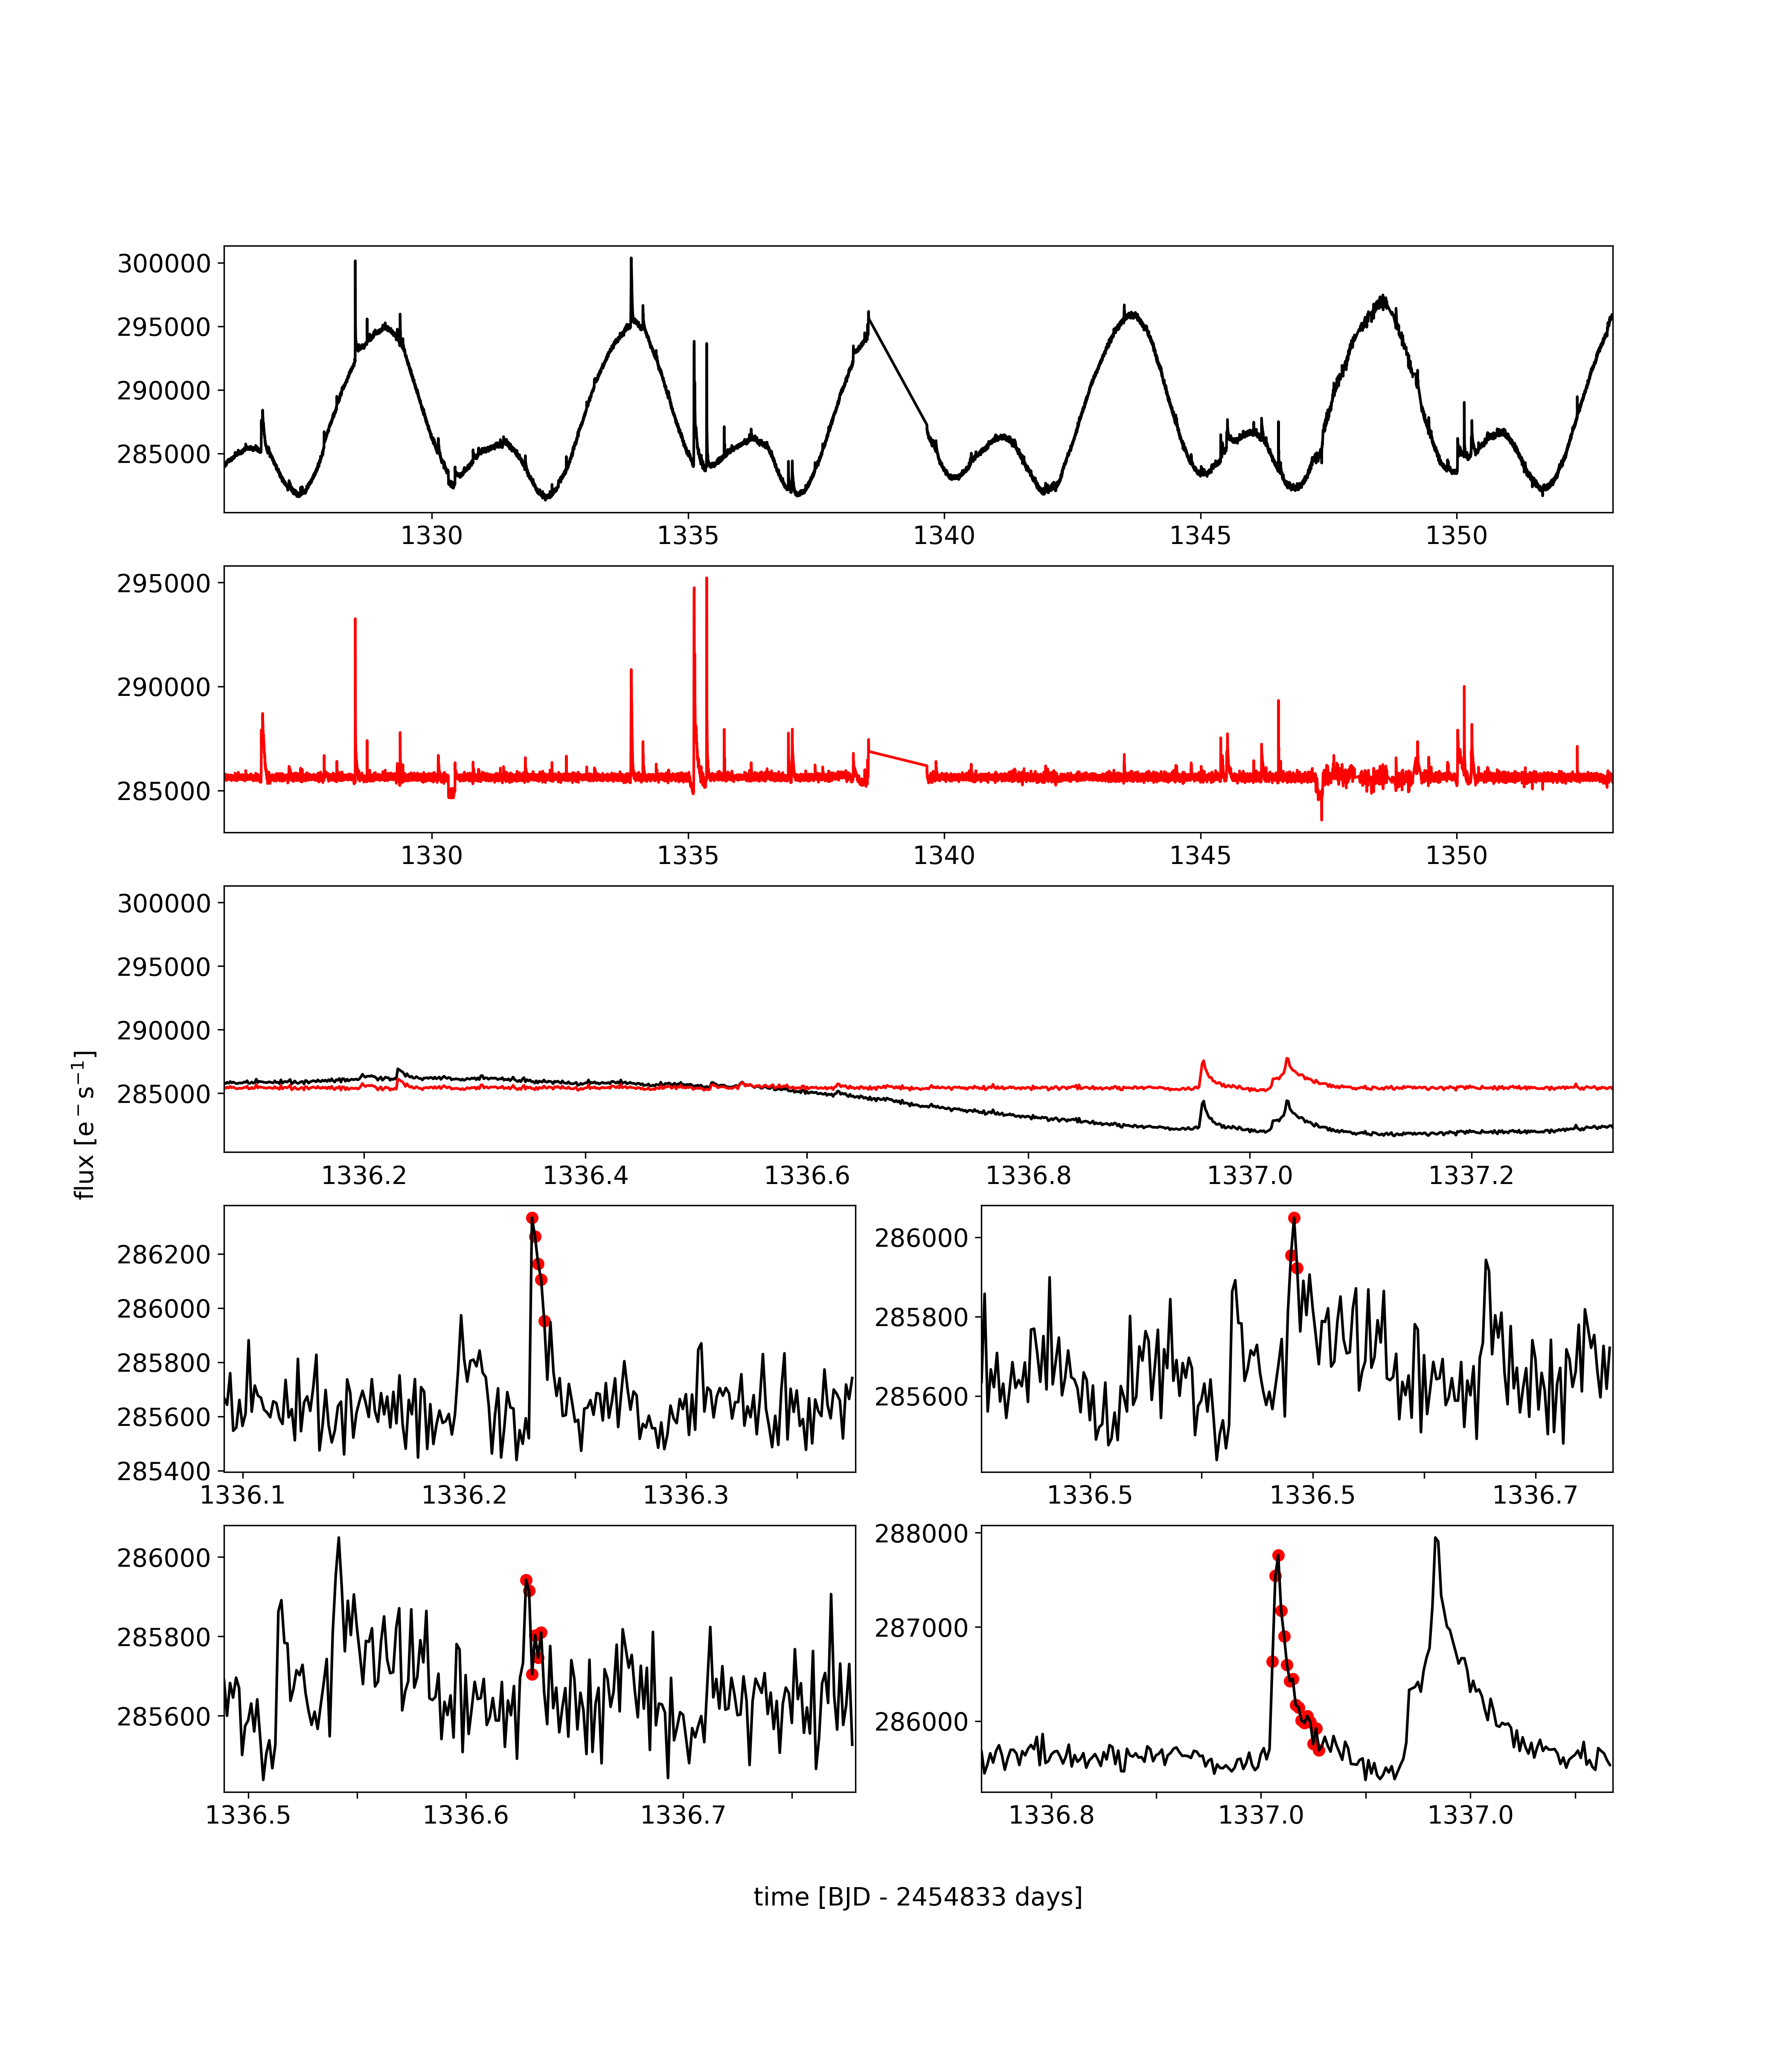
\includegraphics[width=\hsize]{figures/aumic_illustrate_flares.png} 
\caption{Subset of flares detected in the TESS light curve of AU Mic, Sector 1.}
\label{fig:illustrate_detrend}
\end{figure*}

%\begin{figure}
%\includegraphics[width=\hsize]{figures/sigma_clipping.png} 
%\caption{Padded sigma clipping technique applied to 4-data point flare.}
%\label{fig:illustrate_clipping}
%\end{figure}
% Noise estimat

\subsection{Flare catalog}
\label{sec:flarecatalog}
We confirmed 75 flares in Sector 1 and 114 in Sector 27, fewer than the XXXX and XXXX reported in~\citet{martioli2021}.

\section{Flare rate variation with rotational and orbital phases}
\label{sec:phases}
\begin{figure*}
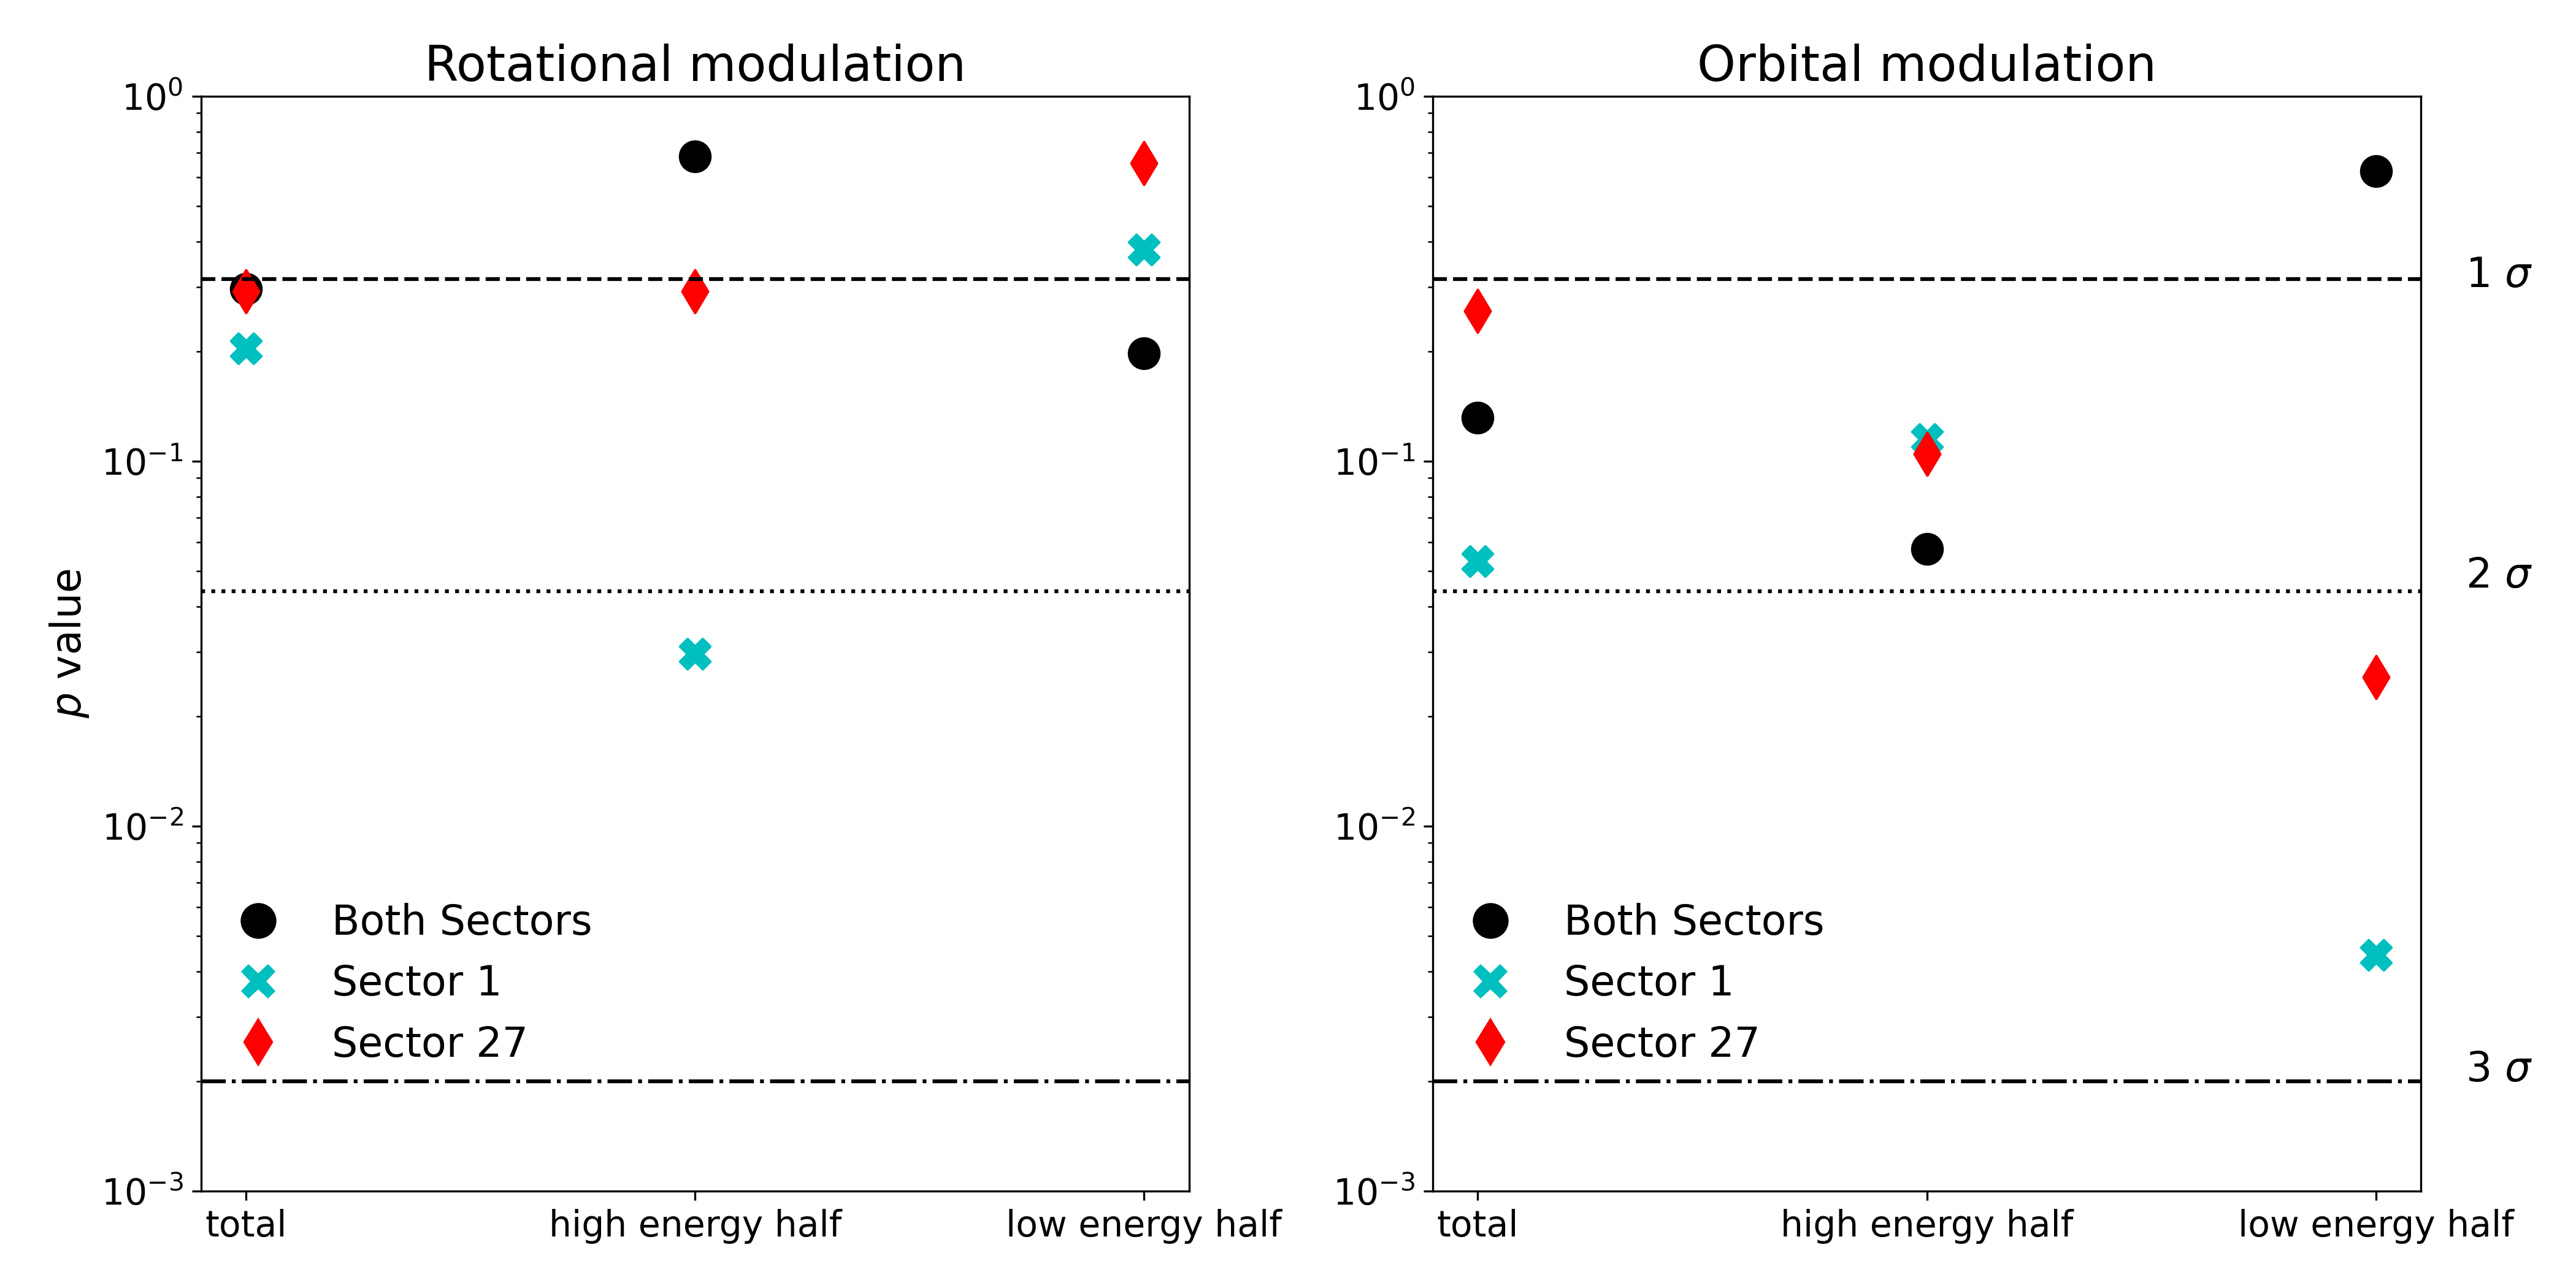
\includegraphics[width=\hsize]{figures/2021_06_09_AUMic_KStests_meta.png} 
\caption{Kolmogorov-Smirnov test results. Black circles, cyan crosses and red diamonds indicate $p$-values obtained using the both available light curve, only the 2-min light curve in Sector 1, or only the 20s light curve in Sector 27, respectively. Each subfigure shows the $p$-values obtained either using the full sample of flares, or 50\% of the most energetic, or 50\% of the least energetic flares, respectively. The $1-,\;2-$ and $3-\sigma$ detection levels are indicated as dashed, dotted and dash-dotted horizontal lines. We see no detections at the $3-\sigma$ level with either rotational or orbital modulation.}
\label{fig:kstests}
\end{figure*}
\begin{figure}
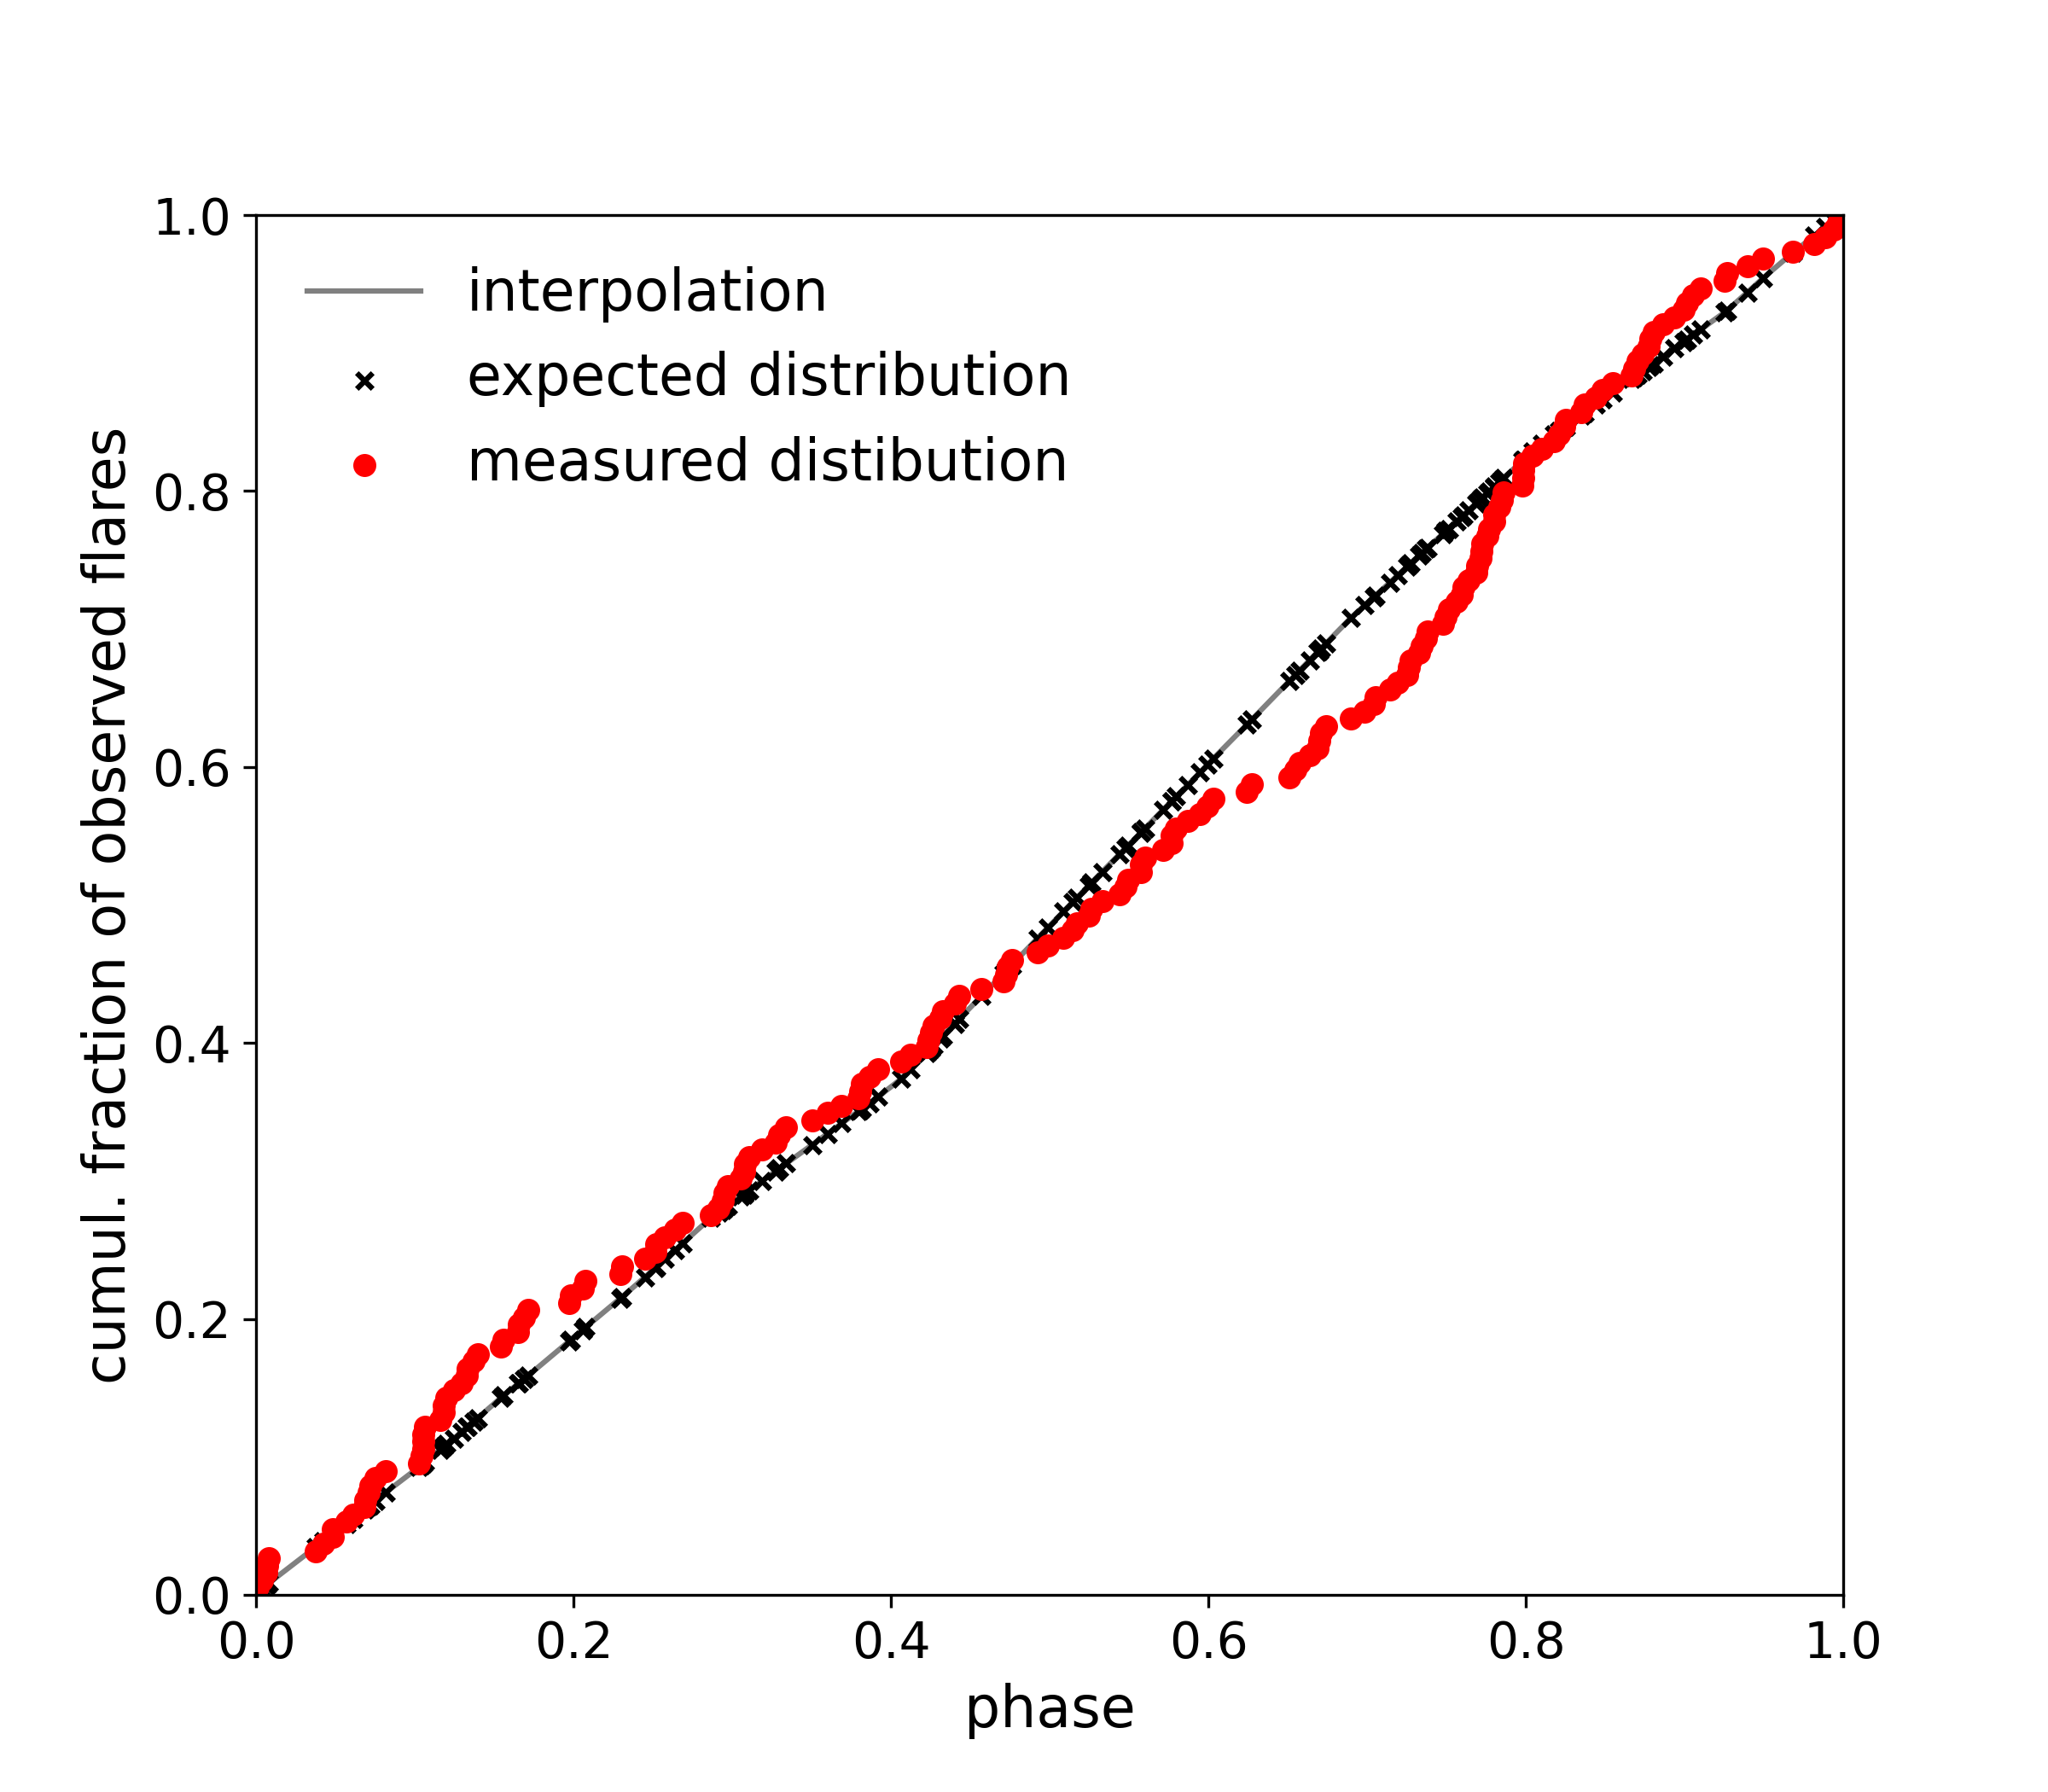
\includegraphics[width=\hsize]{figures/2021_06_08_AUMic_KS_Test_cumdist_total_Both_Sectors_Orbit.png} 
\caption{Cumulative distribution function of flare occurrences as a function of the orbital phase of AU Mic b. Black crosses and black line: The expected distribution with crosses indicating the expected cumulative fraction of observed flares at a given orbital phase. Red circles: Measured cumulative fraction of observed flares as a function of orbital phase. The K-S statistic is defined as the largest absolute vertical distance between the red and the black distribution.}
\label{fig:cumdist}
\end{figure}


\begin{figure}
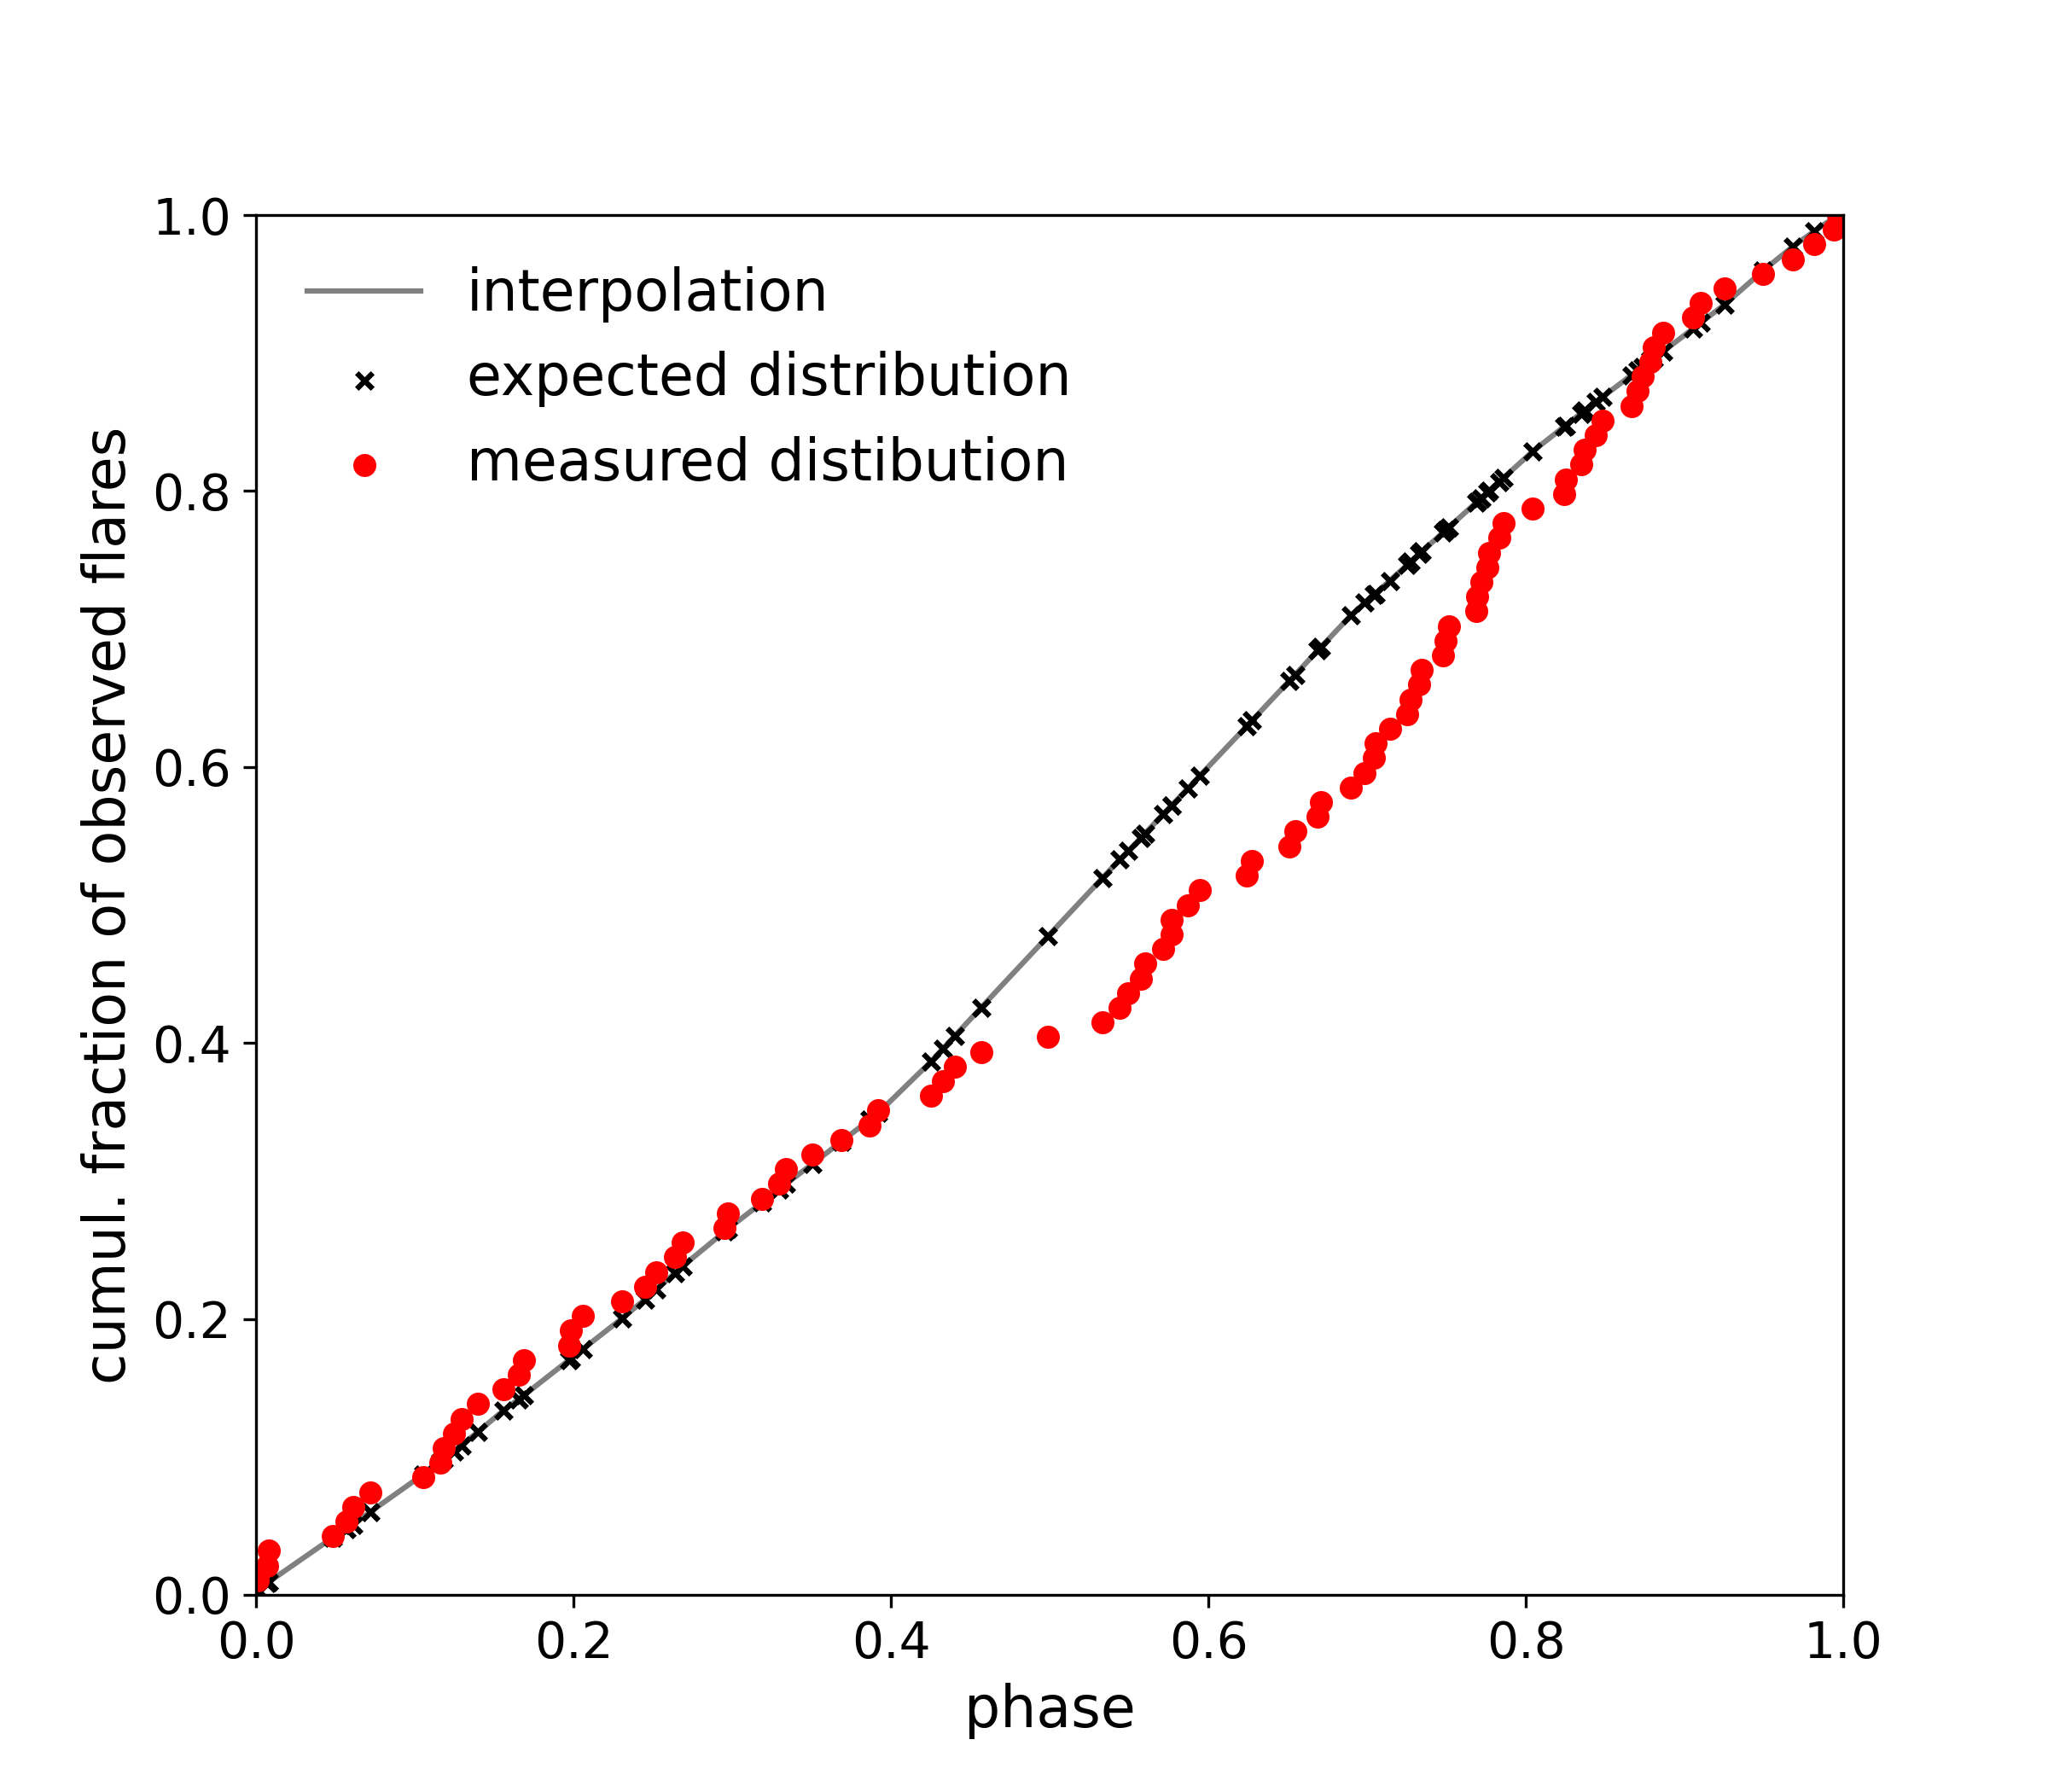
\includegraphics[width=\hsize]{figures/2021_06_09_AUMic_KS_Test_cumdist_high_energy_half_Both_Sectors_Orbit.png} 
\caption{Cumulative distribution function of flare occurrences as a function of the orbital phase of AU Mic b, using the most energetic half of the full flare sample. Colors and symbols are the same as in Fig~\ref{fig:cumdist}}
\label{fig:cumdisthigh}
\end{figure}
\begin{figure}
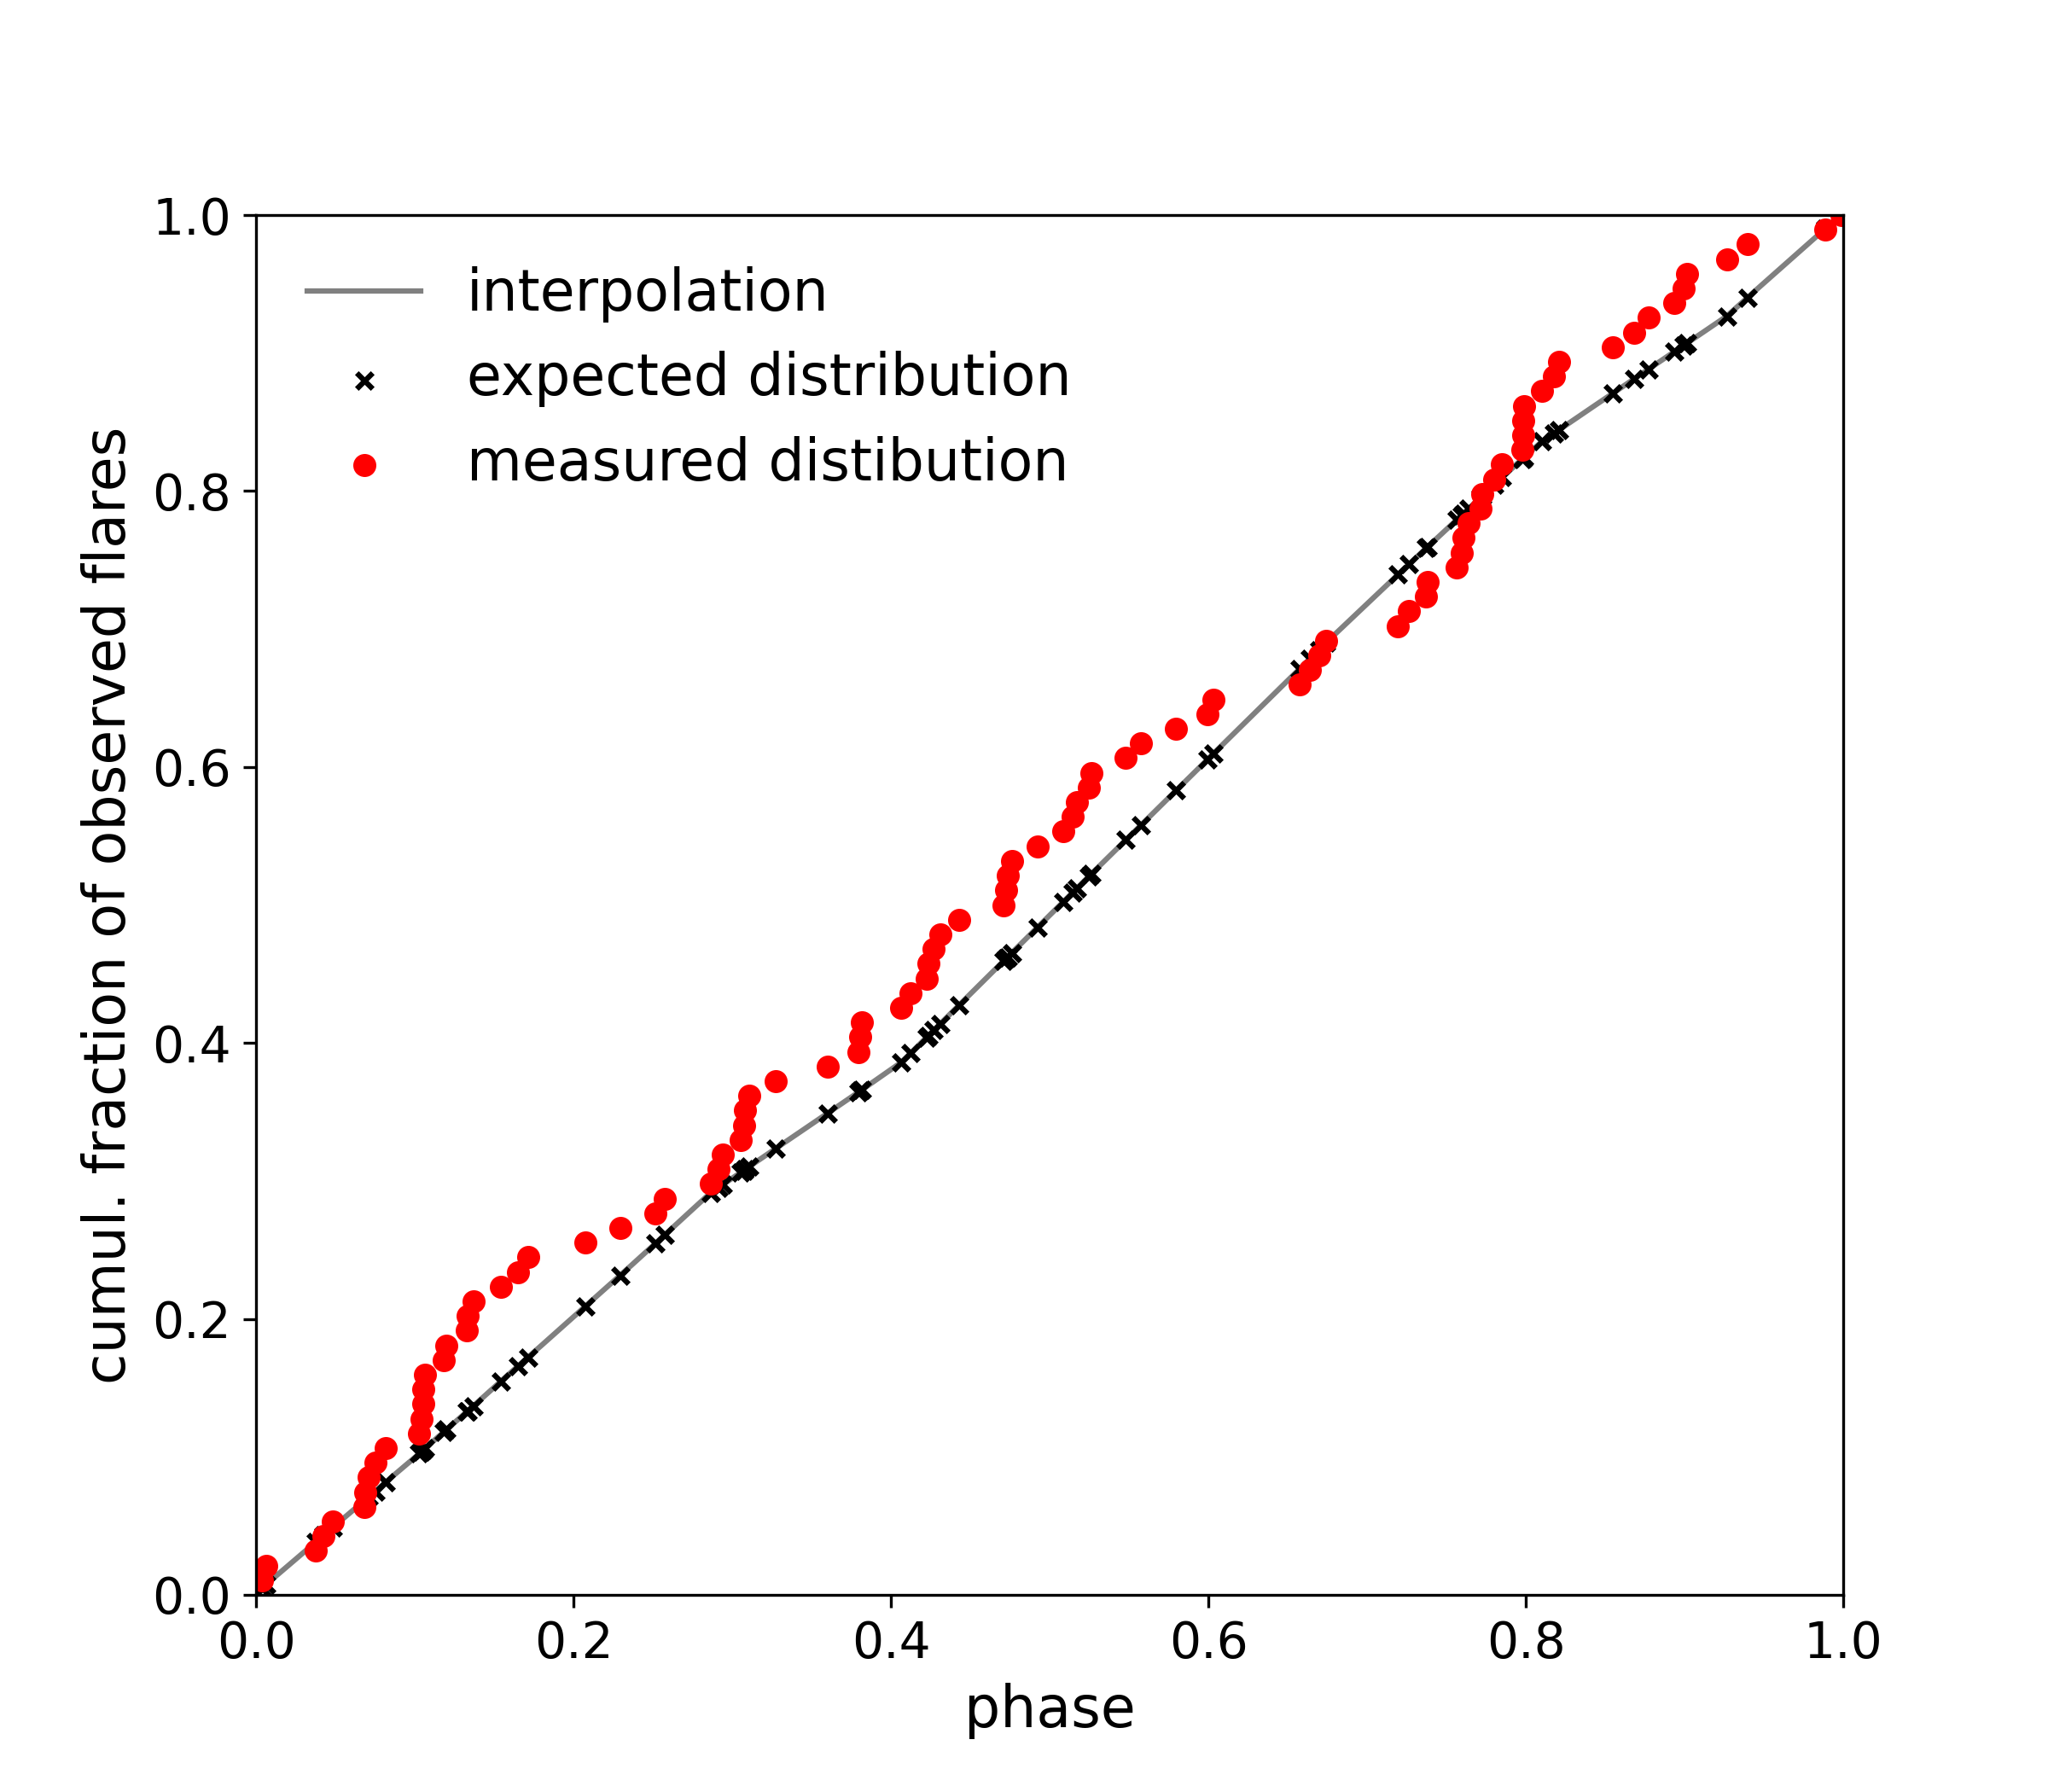
\includegraphics[width=\hsize]{figures/2021_06_09_AUMic_KS_Test_cumdist_low_energy_half_Both_Sectors_Orbit.png} 
\caption{Cumulative distribution function of flare occurrences as a function of the orbital phase of AU Mic b, using the least energetic half of the full flare sample. Colors and symbols are the same as in Fig~\ref{fig:cumdist}}
\label{fig:cumdistlow}
\end{figure}

In the following we assume that we analyse $N$ light curves $S_k$ with $k\in [1,N]$ that cover observign periods that do not overlap, and each of which has the same flare detection threshold throughout the observing time of the light curve. However, our method allows that the treshold can vary from light curve to light curve. This is the case for the two Sectors in which AU Mic was observed, because Sector 1 was observed in 2 min cadence, and Sector 27 in 20 s cadence. In the latter, less energetic flares can be detected than in the former.

After having searched all $S_k$ for flares (Setion~\ref{sec:detrendfind}), we calculate the deviation from a uniform flare rate distribution with orbital and rotational phase in five steps:
\begin{enumerate}
\item First, we take all $F$ flare occurrence times in AU Mic and derive their orbital or rotational phases $x_i$ with $x \in [1,F]$. 
\item Then, we sort all $x_i$ by phase in ascending order.
\item For each $x_i$, we calculate the number of flares $\hat{n_i}$ we expect to observe in the phase interval $[x_{i-1}, x_i]$, where $x_0\equiv x_F - 1$ (circular boundary condition). Assuming that flare rates are uniformly distributed, we expect to see
$$\hat{n}_i = \displaystyle\sum_{k=1}^N\dfrac{T_{obs, i, k}}{T_{obs, tot, k}} F_k$$
flares, where $T_{obs, tot, k}$ is the total observing time with TESS in each Sector, and the observing time $T_{obs,i,k}$ per phase interval is
$$T_{obs,i,k}=\displaystyle\sum_{(x>x_{i-1}\, \land \, x<x_i)} \Delta t_k,$$
where we sum all observing times in the phase interval. $\Delta t_k$ denotes the TESS observing cadence (2 min or 20 s). By treating each light curve separately we take into account their different detection thresholds, which allows us to stack flare samples from heterogeneous data. The corresponding measured number of flares in that phase interval is $n_i=1$ per definition.
\item We then calculate the cumulative frequencies of expected and measured flares as:
$$f(<i) = \dfrac{1}{F}\displaystyle\sum_{j=i}^{i}n_j= \dfrac{i}{F}$$
$$\hat{f}(<i) =  \dfrac{1}{F}\displaystyle\sum_{j=0}^{i}\hat{n}_j = \dfrac{1}{F}\displaystyle\sum_{j=0}^{i}\displaystyle\sum_{k=1}^N\dfrac{T_{obs, j, k}}{T_{obs, tot, k}} F_k$$
\item Finally, we perform a two-tailed one-sample Kolmogorov-Smirnov (K-S) test to check if our observation $f(<i)$ leads us to reject the uniform distribution hypothesis represented by $\hat{f}(<i)$.
\end{enumerate}
We show both distributions for the complete sample of orbital flare phases that was passed to \texttt{scipy.stats.ks\_1samp} in Fig.~\ref{fig:cumdist}. The expected distribution is not a straight line because the different phase coverages combined with different detection thresholds of the light curves are accounted for in the derivation of the distribution (step (iii)). 

The resulting $p$-values obtained from the K-S test are shown in Fig.~\ref{fig:kstests}. Because AU Mic is seen nearly equator-on, the rotational phase diagrams are consistent with a uniform distribution of flares with stellar longitude (left panel in Fig.~\ref{fig:kstests}). 

The observed distribution of flares deviates by $1-2\sigma$ from a uniform distribution of flares with orbital period, which might be attributed to flaring SPI (right panel in Fig.~\ref{fig:kstests}). This effect is stronger for more energetic half~(Fig.~\ref{fig:cumdisthigh}), but disappears for the least energetic half of the flare sample~(Fig.~\ref{fig:cumdistlow}). The deviation seen in the cumulative distribution in the full sample also becomes more pronounced in the more energetic subsample~(Fig.~\ref{fig:cumdisthigh}). 

The TESS data comprise $<50$ days of observations, i.e., covering only abbout $5.7$ orbits of AU Mic b. The same magnitude of deviation would be significant at the $99\%$ or  $99.9\%$ confidence level if the observation baseline could be extended by  62.7 d ($7.4\;P_{orb}$), or 117.3 d ($13.9\;P_{orb}$), respectively. Therefore, longer monitoring of AU Mic in the optical could clarify whether SPI is present or not. In contrast to spot-induced modulation of flare occurrence rates that can only be substantiated for spots that are sufficiently long-lived, orbital modulation can use combined data from many observational campaigns. 
\begin{table}
\caption{Required observing time in days for a $99\%$ or $99.9\%$ confidence level detection of orbital phase dependent flare rates. Predictions are based on the K-S statistic obtained from the flare rates in Sectors 1, 27, and the combined sample. The required time is shorter for 20 s cadence observations than for 2 min cadence.}
\centering
\input{tables/prediction.tex}
\label{tab:prediction}
\end{table}
What fraction of flares stem from SPI? How many flares do we need to observe for this fraction to become significant, i.e., so that error on flare frequency $<<$ number of SPI flares?
\\
Even if we get a significant deviation, it is not proof that it stems from flaring SPI. However, it would allow us to more concretely model the flaring behaviour. And second, if we are correct to assume that the spot configuration in AU Mic varies across time, and the flaring regions appear and disappear on sufficiently short time scales, stacking temporally separated observations will average out effects of rotational variability. The spot pattern in Sector 1 is more stable than in Sector 27~\citep{martioli2021}
\section{Discussion and Conclusions}
\label{sec:discussion}
%\subsection{Were our results expected?}
No correlation with rotation period, consistent with literature~\citep{doyle2018, doyle2019}

The data cover only about 45 days of observations, that is, ~5 orbits of AU Mic b, and ~8 rotations of the star.

\citet{kavanagh2021} predict magnetic SPI with AU Mic b to be observable as ECMI originating from the star.  

\citet{fischer2019} did not find any sign of flaring SPI in TRAPPIST-1  

We find weak hints of flaring SPI, and no rotational variability in flare occurrence rates in AU Mic. If the marginal oribital phase correlated signal can, however, be interpreted as emerging SPI signal, we argue that further monitoring of AU Mic may reveal the interaction. Using the method introduced here, a longer observing baseline with TESS, covering additional 30--120 days in 2 min cadence, and light curves from other surveys, optical or in other flare-sensitive wavelength bands, can be stacked consistently to confirm or reject the flaring SPI hypothesis for AU Mic. It would also allow us to measure the strength of, or find an upper limit to, the interaction, which is difficult to constrain in theory~\citep{strugarek2019}. We expect that long gaps on time scales of months to years betweeen consecutive light curves help to average out any confounding rotational variability signal, but should leave the SPI signal fully intact.

% 

In an upcoming study, we will be applying the methods of flare finding and orbital phase analysis presented here to a large sample of star-planet systems with known close-in planets to increase the total number of orbits covered and to probe the effects of orbital distance, mass (ratio) and others.
\section*{Acknowledgements}
We made use of numpy~\citep{numpy2020} and pandas~\citep{pandas2010,pandas2020software}

This research has made use of the SIMBAD database, operated at CDS, Strasbourg, France~\citep{wenger2000}

%This publication makes use of data products from the Two Micron All Sky Survey, which is a joint project of the University of Massachusetts and the Infrared Processing and Analysis Center/California Institute of Technology, funded by the National Aeronautics and Space Administration and the National Science Foundation.

%This work has made use of data from the European Space Agency (ESA) mission {\it Gaia} (\url{https://www.cosmos.esa.int/gaia}), processed by the {\it Gaia} Data Processing and Analysis Consortium (DPAC, \url{https://www.cosmos.esa.int/web/gaia/dpac/consortium}). Funding for the DPAC has been provided by national institutions, in particular the institutions participating in the {\it Gaia} Multilateral Agreement.
%%%%%%%%%%%%%%%%%%%%%%%%%%%%%%%%%%%%%%%%%%%%%%%%%%

%%%%%%%%%%%%%%%%%%%% REFERENCES %%%%%%%%%%%%%%%%%%

% The best way to enter references is to use BibTeX:

\bibliographystyle{mnras}
\bibliography{bibliography}


% Alternatively you could enter them by hand, like this:
% This method is tedious and prone to error if you have lots of references
%\begin{thebibliography}{99}
%\bibitem[\protect\citeauthoryear{Author}{2012}]{Author2012}
%Author A.~N., 2013, Journal of Improbable Astronomy, 1, 1
%\bibitem[\protect\citeauthoryear{Others}{2013}]{Others2013}
%Others S., 2012, Journal of Interesting Stuff, 17, 198
%\end{thebibliography}

%%%%%%%%%%%%%%%%%%%%%%%%%%%%%%%%%%%%%%%%%%%%%%%%%%

%%%%%%%%%%%%%%%%% APPENDICES %%%%%%%%%%%%%%%%%%%%%

%\appendix
%
%\section{Some extra material}
%
%additional material which would interrupt the flow of the main paper


%%%%%%%%%%%%%%%%%%%%%%%%%%%%%%%%%%%%%%%%%%%%%%%%%%


% Don't change these lines
\bsp	% typesetting comment
\label{lastpage}
\end{document}

% End of mnras_template.tex
